\documentclass[handout]{beamer}

\usepackage[utf8]{inputenc}
\usepackage{default}
\usepackage{graphicx}
\pdfimageresolution=300


\title{OL3-Cesium: 3D for OpenLayers}
\author{Guillaume Beraudo}
\date{FOSS4G Bonn, August 26\textsuperscript{th} 2016}
\subject{Talk OL3-Cesium FOSS4G 2016}

\hypersetup{colorlinks,urlcolor=blue}
\setbeamertemplate{footline}[text line]{%
  \parbox{\linewidth}{\vspace*{-8pt}OL3-Cesium\hfill\insertshortauthor, FOSS4G Bonn 2016}}
\setbeamertemplate{navigation symbols}{}

\begin{document}

  \begin{frame}
    \titlepage
    \begin{center}
      \includegraphics[width=.2\linewidth]{images/foss4g-banner.png}
      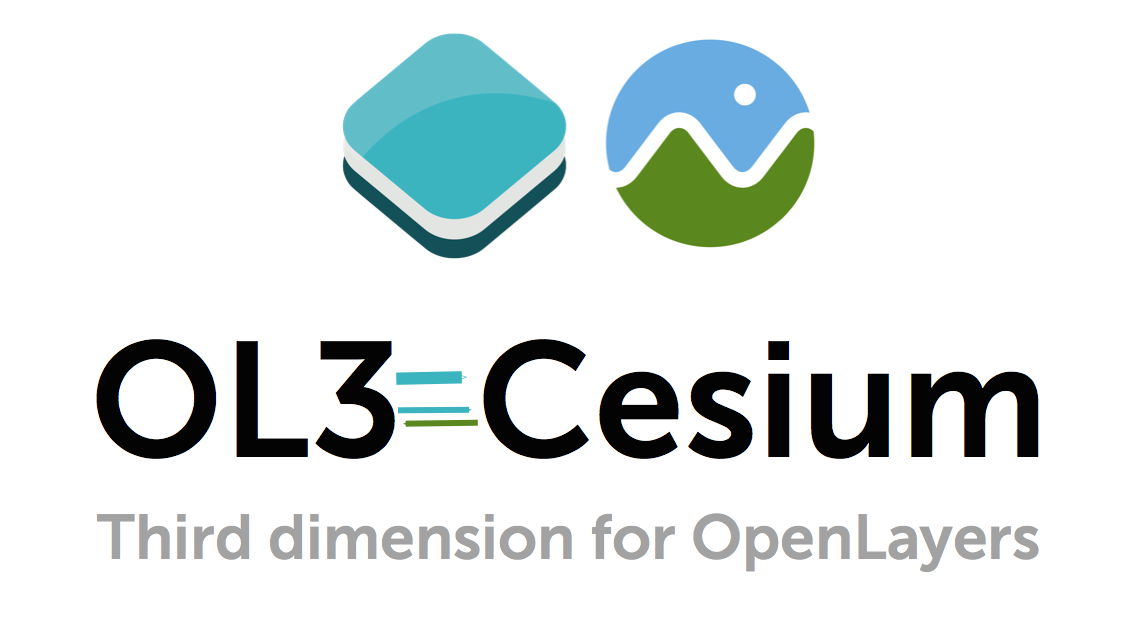
\includegraphics[width=.2\linewidth]{images/ol3-cesium-wide_arrows.png}
      \includegraphics[width=.2\linewidth]{./images/logo_c2c.png}
    \end{center}
  \end{frame}


  \begin{frame}
    \frametitle{About me}
    \begin{itemize}
      \item Senior software engineer at Camptocamp
      \item OL3-Cesium main developer and release manager
      \item OpenLayers 3 and Cesium contributor
      \item On github: \href {https://github.com/gberaudo}{@gberaudo}
      \end{itemize}
  \end{frame}


  \begin{frame}
    \frametitle{OpenLayers 3 - The world is flat!}
    \begin{center}
     \includegraphics[width=.7\linewidth]{./images/flat_earth2.png}
    \end{center}
  \end{frame}


  \begin{frame}
    \frametitle{OpenLayers 3 - The world is flat!}
    \begin{itemize}
      \item Developement since 2013 (2006 for OpenLayers 2)
      \item Raster and vector layers drawn on top of each other
      \item View with arbitrary projection, rotation, resolution, position
      \item Same resolution for all pixels
      \item Flexible, optimized, pixel perfect
      \item \textbf{flat?}
     \end{itemize}
  \end{frame}


  \begin{frame}
    \frametitle{Cesium - The world is a realistic 3D scene}
    \begin{center}
     \includegraphics[width=.7\linewidth]{./images/round_earth2.png}
    \end{center}
% Ajouter le soleil
    \end{frame}


  \begin{frame}
    \frametitle{Cesium - The world is a realistic 3D scene}
    \begin{itemize}
      \item Developement since 2012
      \item Only Mercator and Lonlat (EPSG:3857 and EPSG:4326)
      \item WGS84 ellipsoid
      \item XYZ, terrain, models, lights
      \item WebGL, custom optimized renderer
    \end{itemize}
  \end{frame}


  \begin{frame}
    \frametitle{Cesium - Challenges}
    \begin{itemize}
      \item Vector on (dynamic) terrain
      \item Raster on steep terrain
      \item Trees, planes, bridges, buildings (3D-tiles)
%       Add link to 3D tiles spec?
      \item Needs (lots of) CPU, GPU, bandwidth
    \end{itemize}

% 2D and 3D : somehow different focus and challenges
% How to combine their strength?
   \end{frame}


  \begin{frame}
    \frametitle{OL3-Cesium - The best of all worlds}
    \begin{itemize}
      \item Developement since 2014
      \item Write once, use in 2D and 3D
      \item Receive and give to the community
      \item Start interacting in one world and continue in the other
      \item Easiest path to add 3D to an OpenLayers 3 map
      \item In a nutshell \textbf{it makes a great application awesome}
    \end{itemize}
  \end{frame}


  \begin{frame}
    \frametitle{OL3-Cesium - Ready for prime time}
    \begin{figure}
    \begin{center}
      \includegraphics[width=.6\linewidth]{./images/schweizmobil_vtt_3d3.png}
    \end{center}
    \href {https://map.schweizmobil.ch/?cesium&trackId=2149217&lang=fr&bgLayer=lb&resolution=10.86&X=561417&Y=141893&layers=Bus\%2CWanderland}{SchweizMobil - outdoor application}
    \end{figure}

    \begin{itemize}
      \item Custom 3D terrain - different projections
      \item 3D vector clustering with 30'000 points
      \item Optimized for an high number of users
      \item CPU/GPU resource saving by stopping the render loop
      \item Workaround for lines on terrain
     \end{itemize}
  \end{frame}

  \begin{frame}
    \frametitle{OL3-Cesium - Ready for prime time}
    \begin{figure}
    \begin{center}
      \includegraphics[width=.6\linewidth]{./images/geoadmin_water_catchment_areas.png}
    \end{center}
    \href {https://map.geo.admin.ch}{Geoadmin - Swiss geoportal}
    \end{figure}

    \begin{itemize}
      \item Lazy loading - nice 2D/3D transitions
      \item 3D tiles: buildings, bridges
      \item Own synchronizers (raster $\rightarrow$ vector, different projections)
      \item New points of views
    \end{itemize}
  \end{frame}


  \begin{frame}
    \frametitle{OL3-Cesium - quality / bandwidth}
    \begin{center}
      \includegraphics[width=\linewidth]{./images/schweizmobil_fog.png}
    \end{center}

    \begin{itemize}
     \item \href {https://github.com/gberaudo/ol3-cluster-tool}{Vector clustering}: top quality, some geojsons instead of millions of raster tiles
     \item Fog: reduce details according to distance from the camera
    \end{itemize}
  \end{frame}


  \begin{frame}
    \frametitle{OL3-Cesium - Immersive views}
    View from a mountain trail
    \begin{center}
      \includegraphics[width=\linewidth]{./images/geoadmin_immersive_view.png}
    \end{center}
  \end{frame}


  \begin{frame}
    \frametitle{OL3-Cesium - Immersive views}
    View through a window
    \begin{center}
      \includegraphics[width=\linewidth]{./images/geoadmin_immersive_view_from_home.png}
    \end{center}
  \end{frame}


  \begin{frame}
    \frametitle{Ideas for the future - need founding}
    \begin{itemize}
      \item Lines on terrain workaround (corridor geometries)
        \pause
      \item Integrate 3D vector clustering
        \pause
      \item Client side reprojection
        \pause
      \item Official extruded polygons support
    \end{itemize}
  \end{frame}


  \begin{frame}
    \frametitle{Questions?}
    \vspace{-20pt}\begin{center}
      \includegraphics[width=0.9\linewidth]{images/github_contribute.png}
    \end{center}
    \begin{itemize}
      \item Thanks to OSM, SchweizMobil and swisstopo
        \pause
      \item Thanks to you for listening
        \pause
      \item Danke - Questions?
    \end{itemize}
  \end{frame}


  \begin{frame}
    \frametitle{Future: 3D imagery}
    \begin{center}
      \includegraphics[width=0.6\linewidth]{images/schweizmobil_cesium_steep_raster.png}
    \end{center}
    \begin{itemize}
      \item We need more precision where the terrain is steeper
        \pause
      \item We need multi-view capture of imagery (not just top-down)
    \end{itemize}
  \end{frame}

  \begin{frame}
    \frametitle{Links}
    \begin{itemize}
      \item \href {https://github.com/openlayers/ol3-cesium}{OL3-Cesium}
      \item \href {https://github.com/gberaudo/ol3-cluster-tool}{OL3 cluster Tool}
      \item \href {https://github.com/geoadmin/mf-geoadmin3}{Geoadmin} / \href {https://map.geo.admin.ch}{github}
      \item \href {https://map.schweizmobil.ch}{SchweizMobil}
      \item \href {https://github.com/geo-data/cesium-terrain-builder}{Cesium-terrain-builder heightmap terrain}
      \item \href {https://github.com/geoadmin/3d-forge}{3d-forge quantized terrain}
    \end{itemize}
  \end{frame}

\end{document}
